\section{Experiments}

In this section, we compare \method with state-of-the-art methods for camera pose estimation and 3D reconstruction, analyze efficiency, and conduct ablation studies.
Training details and data are described in~\cref{sec:training},
the evaluation benchmark is defined in~\cref{sec:benchmark},
and inference configuration is specified in~\cref{sec:inference_mode}.


\subsection{Baseline Methods}

We compare \method against three categories of methods:

\paragraph{Offline Feed-Forward Models.}
These methods process all input frames simultaneously using
bidirectional attention, producing globally consistent reconstructions
in a single forward pass but requiring access to the full sequence.
We include VGGT~\cite{wang2025vggt},
DA3~\cite{depthanything3},
Fast3R~\cite{yang2025fast3r},
FastVGGT~\cite{shen2025fastvggt},
and Pi3~\cite{wang2025pi}.

\paragraph{Optimization-Based Methods.}
These methods iteratively refine camera poses and geometry through
explicit optimization objectives such as reprojection error
minimization or bundle adjustment.
They typically achieve high accuracy but at significant computational
cost.
We include DroidSLAM~\cite{teed2021droid},
MegaSAM~\cite{li2025megasam},
and VIPE~\cite{huang2025vipe}.

\paragraph{Streaming Methods.}
These methods process frames causally in a streaming fashion,
predicting poses and depth without access to future frames.
This is the same setting as \method.
We include StreamVGGT~\cite{streamVGGT},
SLAM3R~\cite{liu2025slam3r},
InfiniteVGGT~\cite{yuan2026infinitevggt},
Spann3R~\cite{wang20253d},
Stream3R~\cite{stream3r2025},
CUT3R~\cite{cut3r},
TTT3R~\cite{chen2025ttt3r},
and Wint3R~\cite{li2025wint3r}.
For fair comparison, all streaming methods are evaluated without
resetting their internal state throughout each sequence.




\subsection{Camera Pose Estimation}

\paragraph{Large-Scale Trajectory Estimation on Oxford Spires.}
Oxford Spires is one of the most challenging benchmarks for streaming
pose estimation: sequences span complex indoor-outdoor environments
with abrupt scene transitions (e.g., outdoor courtyards to dark
staircases), revisits to previously observed areas after long temporal
gaps, and large scale variation across the trajectory.
These properties demand both accurate local pose estimation and
long-range global consistency, which are precisely the capabilities
GCA is designed to provide.
We evaluate under two settings to test both aspects.

In the \textit{sparse} setting (320 frames, sampled every 12 frames),
all method categories can run on our hardware, enabling a fair
comparison across offline, optimization-based, and online approaches.
As shown in~\cref{tab:pose_accuracy_short_oxford}, \method
achieves the best results on nearly all metrics.
Despite operating in a streaming online manner, our method surpasses
the strongest offline baselines by a large margin.
\method achieves an AUC@15 of 61.64, substantially exceeding the
best offline method DA3~\cite{depthanything3} (49.84) and more than
doubling VGGT~\cite{wang2025vggt} (23.84).
On trajectory-level accuracy, \method reduces ATE from 12.87
(DA3) and 24.78 (VGGT) to 6.42.
We attribute this to a fundamental limitation of existing offline
methods: they are trained on datasets with a small number of
viewpoints where consecutive frames remain close to each other and
largely observe the same local region.
When confronted with the complex scene transitions and large
viewpoint changes in Oxford Spires, the learned priors fail to
transfer.
Compared with optimization-based methods, which explicitly minimize
reprojection error across frames, \method still achieves superior
performance.
\method outperforms the best optimization-based approach
VIPE~\cite{huang2025vipe} on both pose accuracy
(AUC@15: 61.64 vs.\ 45.35) and trajectory consistency
(ATE: 6.42 vs.\ 10.52).
VIPE relies on iterative bundle adjustment and is computationally
expensive; in contrast, \method achieves this accuracy in a single
forward pass.
Among online streaming methods, the performance gap is even more
pronounced.
All competing approaches suffer from severe memory forgetting: as
the sequence progresses, they lose track of previously observed
geometry, leading to accumulated drift.
The best online competitor, CUT3R~\cite{cut3r}, achieves an AUC@15
of only 5.98 and ATE of 18.16, while \method achieves 61.64 and
6.42 respectively, a $10\times$ improvement in pose accuracy and
$2.8\times$ reduction in trajectory error
(see~\cref{fig:traj_results}(a) for qualitative comparison).

\begin{table}[t]
\centering
\caption{\textbf{Pose and trajectory accuracy comparison on Oxford Spires (sparse setting).}
Our method achieves the best performance on most metrics among prior offline, optimization-based, and online methods. The \textbf{best} and \underline{second best} results are marked.}
\label{tab:pose_accuracy_short_oxford}
\begin{tabular}{l c ccccc}
\toprule
Methods & Type & AUC@15 $\uparrow$ & AUC@30 $\uparrow$ & ATE $\downarrow$ & RPE-trans $\downarrow$ & RPE-Rot $\downarrow$ \\
\midrule
Fast3R~\cite{yang2025fast3r}      & offline & 1.20 & 2.99 & 34.80 & 8.21 & 59.51 \\
VGGT~\cite{wang2025vggt}& offline & 23.84 & 35.09& 24.78 & 8.87 & 22.79\\
DA3~\cite{depthanything3}      & offline & \underline{49.84} & \underline{56.68} & 12.87 & 3.22 & 16.17 \\
FastVGGT~\cite{shen2025fastvggt} & offline & 21.68 & 34.64 & 22.43 & 7.25 & 16.12 \\
Pi3~\cite{wang2025pi} & offline & 38.64 & 48.65 & 14.03 & 2.58 & 10.33 \\
\midrule
DroidSLAM~\cite{teed2021droid}& optim & 8.58 & 21.41 & 21.84 & 1.02 & 6.90 \\
MegaSAM~\cite{li2025megasam}& optim & 15.91 & 28.03 & 13.80 & \underline{0.76} & 7.24 \\
VIPE~\cite{huang2025vipe}& optim & 45.35 & 51.88 & \underline{10.52} & \textbf{0.43} & \underline{5.98} \\
\midrule
StreamVGGT~\cite{streamVGGT}& online & 10.91 & 17.04 & 28.41 & 6.35 & 16.28 \\
SLAM3R~\cite{liu2025slam3r}& online & 1.67 & 5.10 & 29.69 & 7.57 & 27.50 \\
InfiniteVGGT~\cite{yuan2026infinitevggt} & online & 10.25 & 16.33 & 30.49 & 5.72 & 15.01 \\
Spann3R~\cite{wang20253d} & online & 2.06 & 5.09 & 32.12 & 3.54 & 14.37 \\
Stream3R-w~\cite{stream3r2025}      & online & 6.56 & 11.03 & 33.03 & 4.73 & 16.79 \\
Stream3R~\cite{stream3r2025}      & online & 9.67 & 15.21 & 29.58 & 6.67 & 16.90 \\
CUT3R~\cite{cut3r}    & online & 5.98 & 14.95 & 18.16 & 1.17 & 7.18 \\
TTT3R~\cite{chen2025ttt3r}    & online & 13.92 & 25.90 & 19.35 & 2.28 & 13.30 \\
Wint3R~\cite{li2025wint3r}      & online & 11.61 & 23.42 & 21.10 & 1.62 & 6.27 \\
\midrule
\method (Ours)  & online & \textbf{61.64} & \textbf{75.16} & \textbf{6.42} & 1.01 & \textbf{3.70} \\
\bottomrule
\end{tabular}
\end{table}

In the \textit{dense} setting (full 3,840 frames), we stress-test
long-sequence streaming capabilities
(\cref{tab:pose_accuracy_long_oxford}).
This setting is particularly revealing: as the trajectory length
increases from 320 to 3,840 frames, most feed-forward methods degrade
dramatically due to accumulated drift.
CUT3R's ATE rises from 18.16 to 32.47 ($1.8\times$ increase), and
Wint3R degrades from 21.10 to 32.90.
In contrast, \method maintains consistently low error
(6.42 $\to$ 7.11), with only a marginal increase of 0.69 over a
$12\times$ longer sequence.
This demonstrates that the three-level context structure of
GCA (anchor, trajectory memory, and local window) effectively
preserves long-range geometric consistency without explicit
optimization or loop closure.
Notably, \method achieves competitive inference speed at 20.29
FPS while maintaining the best trajectory accuracy among all
streaming methods.

\begin{table}[t]
\centering
\caption{\textbf{Sparse vs.\ dense trajectory accuracy on Oxford Spires.}
We compare ATE under the sparse (320 frames) and dense (3,840 frames) settings.
$\Delta$ATE measures the degradation from sparse to dense.
\method maintains near-constant accuracy while competing methods degrade significantly.
The \textbf{best} and \underline{second best} results are marked.}
\label{tab:pose_accuracy_long_oxford}
\setlength{\tabcolsep}{10pt}
\begin{tabular}{lcccccc}
\toprule
 & CUT3R & TTT3R & Wint3R & Inf.-VGGT & Stream3R-w & \method \\
\midrule
ATE$_{\text{sparse}}$ $\downarrow$ & 18.16 & 19.35 & 21.10 & 30.49 & 33.03 & \textbf{6.42} \\
ATE$_{\text{dense}}$ $\downarrow$  & 32.47\rlap{\scriptsize{\textcolor{red}{~(+14.31)}}} & \underline{25.05}\rlap{\scriptsize{\textcolor{red}{~(+5.70)}}} & 32.90\rlap{\scriptsize{\textcolor{red}{~(+11.80)}}} & 31.75\rlap{\scriptsize{\textcolor{red}{~(+1.26)}}} & 33.73\rlap{\scriptsize{\textcolor{red}{~(+0.70)}}} & \textbf{7.11}\rlap{\scriptsize{\textcolor{green!50!black}{~(+0.69)}}} \\
\midrule
FPS $\uparrow$ & \textbf{29.21} & 28.97 & 3.88 & 7.78 & 13.66 & 20.29 \\
\bottomrule
\end{tabular}
\end{table}

\paragraph{Generalization on Diverse Benchmarks.}
To verify that the strong performance on Oxford Spires is not specific
to large-scale outdoor trajectories, we evaluate on three additional
benchmarks that cover fundamentally different scales and scene types:
ETH3D~\cite{schops2017multi} (mixed indoor and outdoor scenes with
laser-scanned ground-truth depth),
7-Scenes~\cite{shotton2013scene} (room-scale RGB-D sequences with
textureless surfaces and significant motion blur),
and Tanks and Temples~\cite{Knapitsch2017} (outdoor multi-view
captures of large structures).
As shown in~\cref{tab:pose_accuracy_short}, \method consistently
outperforms all competing streaming methods by a substantial margin
across all three datasets and all metrics.
\begin{figure}[H]
    \centering
    \vspace{-2em}
    \textbf{(a)} Comparison with SOTA offline and optimization-based methods on Oxford-Spires \\[2pt]
    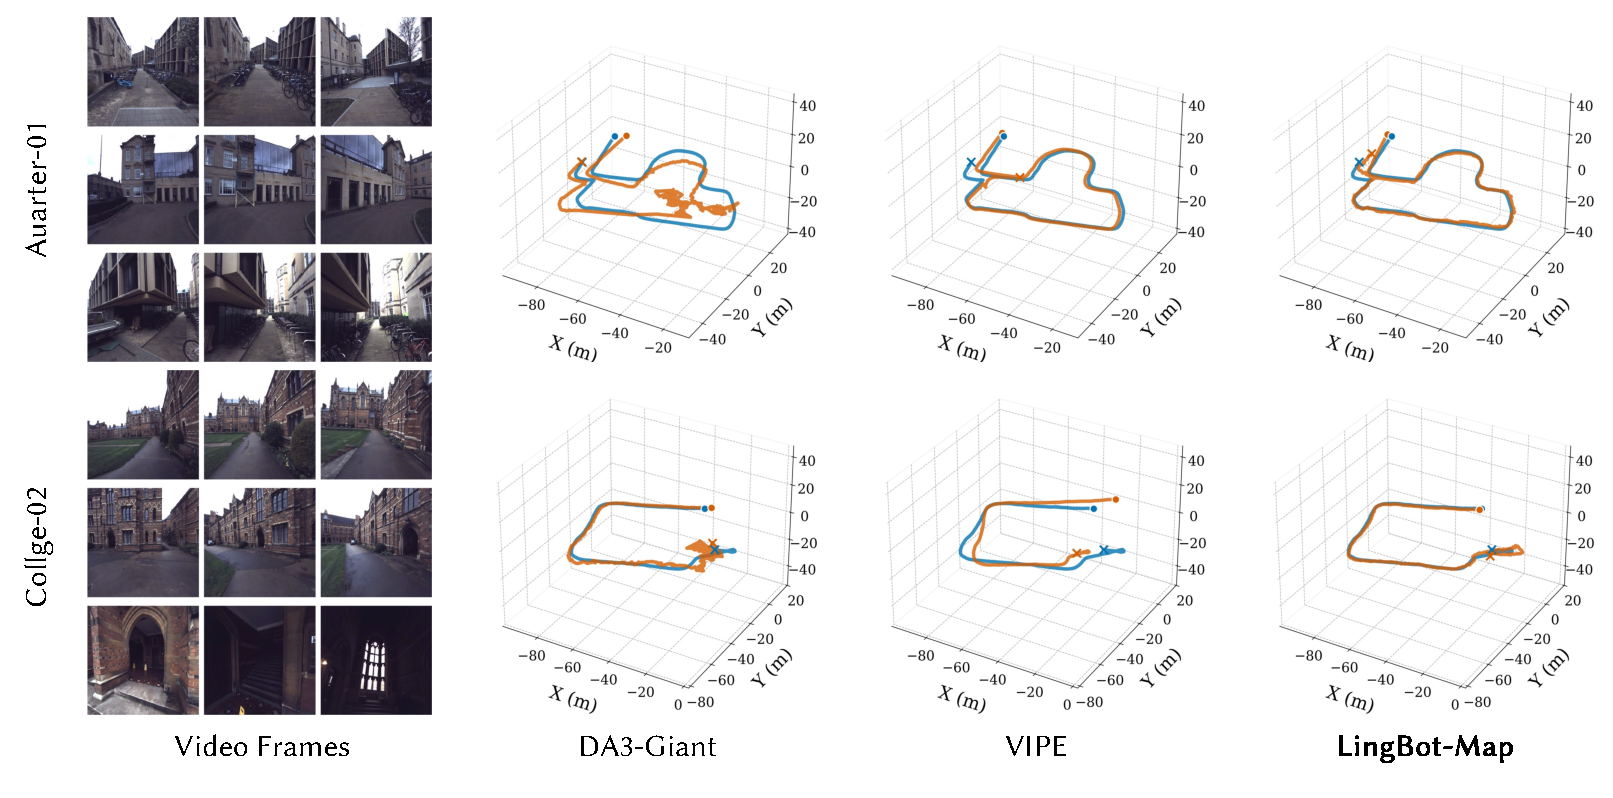
\includegraphics[width=0.9\textwidth]{figures/traj_comparison1.pdf}

    \vspace{3pt}

    \textbf{(b)} Comparison with SOTA streaming methods across diverse scenes \\[2pt]
    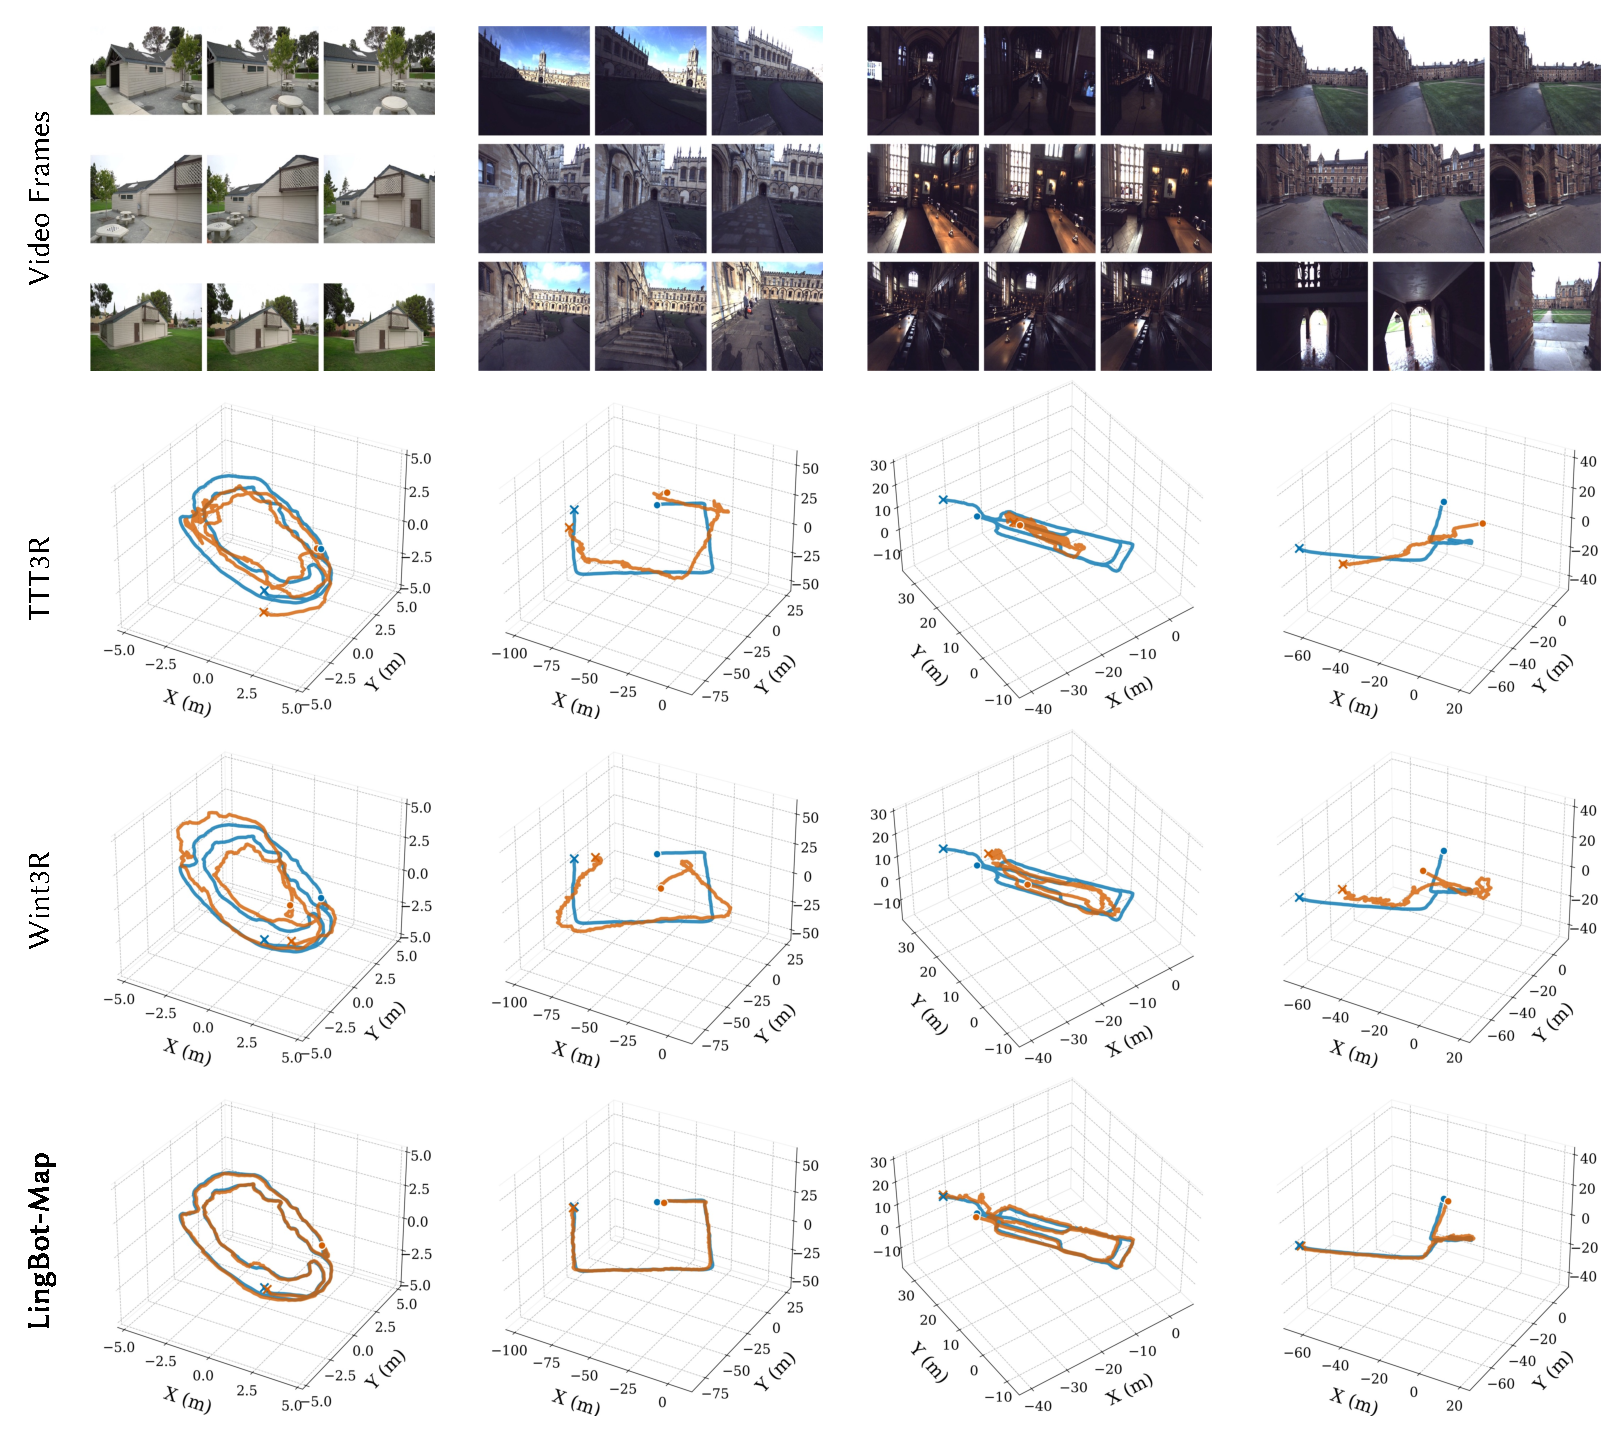
\includegraphics[width=0.9\textwidth]{figures/traj_comparison2.pdf}

    \definecolor{gtcolor}{RGB}{31, 119, 180}
    \definecolor{predcolor}{RGB}{255, 127, 14}

    \caption{\textbf{Trajectory comparison.}
    (a)~On Oxford-Spires, LingBot-Map even outperforms bidirectional (DA3-Giant), and optimization-based (ViPE) methods, accurately preserving trajectories during complex outdoor-to-indoor transitions and dark staircases.
    (b)~Across Tanks and Temples and additional Oxford-Spires scenes, our method consistently produces accurate trajectories while competing streaming methods suffer from severe drift.
    \textcolor{gtcolor}{Ground truth} in blue, \textcolor{predcolor}{predicted} in orange; start~{\textbullet}, end~\textbf{\texttimes}.}
    \label{fig:traj_results}
    \vspace{-8pt}
\end{figure}


On Tanks and Temples, \method achieves an AUC@30 of 92.80 and ATE of
0.20, improving over the runner-up Stream3R (AUC@30: 81.33, ATE: 0.76)
by $+11.47$ AUC points and $3.8\times$ lower ATE.
On ETH3D, our ATE of 0.22 is nearly $4\times$ lower than the
second-best Wint3R (0.86), indicating that our model handles both the
precise indoor geometry and the broader outdoor structures in this
dataset.
On 7-Scenes, \method achieves the lowest ATE of 0.08, confirming
robust performance even on room-scale indoor scenes, where the main
challenges are textureless walls, repetitive structures, and
heavy motion blur rather than trajectory length.
Taken together, these results demonstrate that \method is not a
specialist for any particular scenario but a general-purpose streaming
pose estimator that scales from small rooms to city-scale environments.

Qualitative trajectory comparisons are shown in~\cref{fig:traj_results}.
In part~(a), on Oxford Spires, \method accurately tracks the camera
through complex outdoor-to-indoor transitions and dark staircases,
while DA3-Giant and ViPE both exhibit significant trajectory
drift.
In part~(b), across Tanks and Temples and additional Oxford Spires
scenes, competing streaming methods (TTT3R, Wint3R) produce
trajectories that progressively diverge from the ground truth, whereas
\method consistently maintains close alignment throughout the full
sequence.






\begin{table}[t]
\centering
\caption{\textbf{Pose and trajectory accuracy comparison on ETH3D, 7-Scenes, and Tanks \& Temples.}
Results on ETH3D, 7-Scenes, and Tanks \& Temples show that our method achieves the best performance across all datasets. The \textbf{best} and \underline{second best} results are marked.}
\label{tab:pose_accuracy_short}
\resizebox{\textwidth}{!}{%
\begin{tabular}{l c ccc ccc ccc}
\toprule
\multirow{2}{*}{Methods} & \multirow{2}{*}{Type} &
\multicolumn{3}{c}{ETH3D} &
\multicolumn{3}{c}{7-Scenes} &
\multicolumn{3}{c}{Tanks \& Temples} \\
\cmidrule(lr){3-5}\cmidrule(lr){6-8}\cmidrule(lr){9-11}
 &  & Auc3 $\uparrow$ & Auc30 $\uparrow$ & ATE $\downarrow$ & Auc3 $\uparrow$ & Auc30 $\uparrow$ & ATE $\downarrow$ & Auc3 $\uparrow$ & Auc30 $\uparrow$ & ATE $\downarrow$ \\
\midrule
SLAM3R~\cite{liu2025slam3r}& online & 1.46 & 22.95 & 1.98 & 4.79 & 66.92 & 0.11 & 2.87 & 47.92 & 1.42 \\
Spann3R~\cite{wang20253d} & online & 1.13 & 23.02 & 2.10 & 2.79 & 57.87 & 0.20 & 2.22 & 32.22 & 2.11 \\
InfiniteVGGT~\cite{yuan2026infinitevggt} & online & 12.00 & 62.20 & 1.46 & 8.45 & 73.40 & 0.12 & 21.69 & 77.76 & 1.00 \\
CUT3R~\cite{cut3r}    & online & 10.63 & 57.77 & 1.43 & 1.50 & 42.44 & 0.29 & 1.71 & 25.19 & 1.79 \\
TTT3R~\cite{chen2025ttt3r}    & online & 9.98 & 56.12 & 1.22 & 5.52 & 71.23 & \underline{0.10} & 9.01 & 71.30 & \underline{0.66} \\
Wint3R~\cite{li2025wint3r}      & online & 11.31 & 58.71 & \underline{0.86} & 2.74 & 63.02 & 0.12 & 3.84 & 57.85 & 0.88 \\
Stream3R~\cite{stream3r2025}      & online & \underline{13.73} & \underline{64.76} & 1.67 & \underline{9.31} & \underline{73.70} & \underline{0.10} & \underline{39.27} & \underline{81.33} & 0.76 \\
Stream3R-w~\cite{stream3r2025}      & online & 9.00 & 58.69 & 1.71 & 7.47 & 61.70 & 0.25 & 24.69 & 72.30 & 1.22 \\
\method (Ours)      & online & \textbf{27.79} & \textbf{86.20} & \textbf{0.22}  & \textbf{12.63} & \textbf{78.59} & \textbf{0.08} & \textbf{45.80} & \textbf{92.80} & \textbf{0.20} \\
\bottomrule
\end{tabular}%
}
\end{table}

 \begin{figure}[t!]
    \centering
    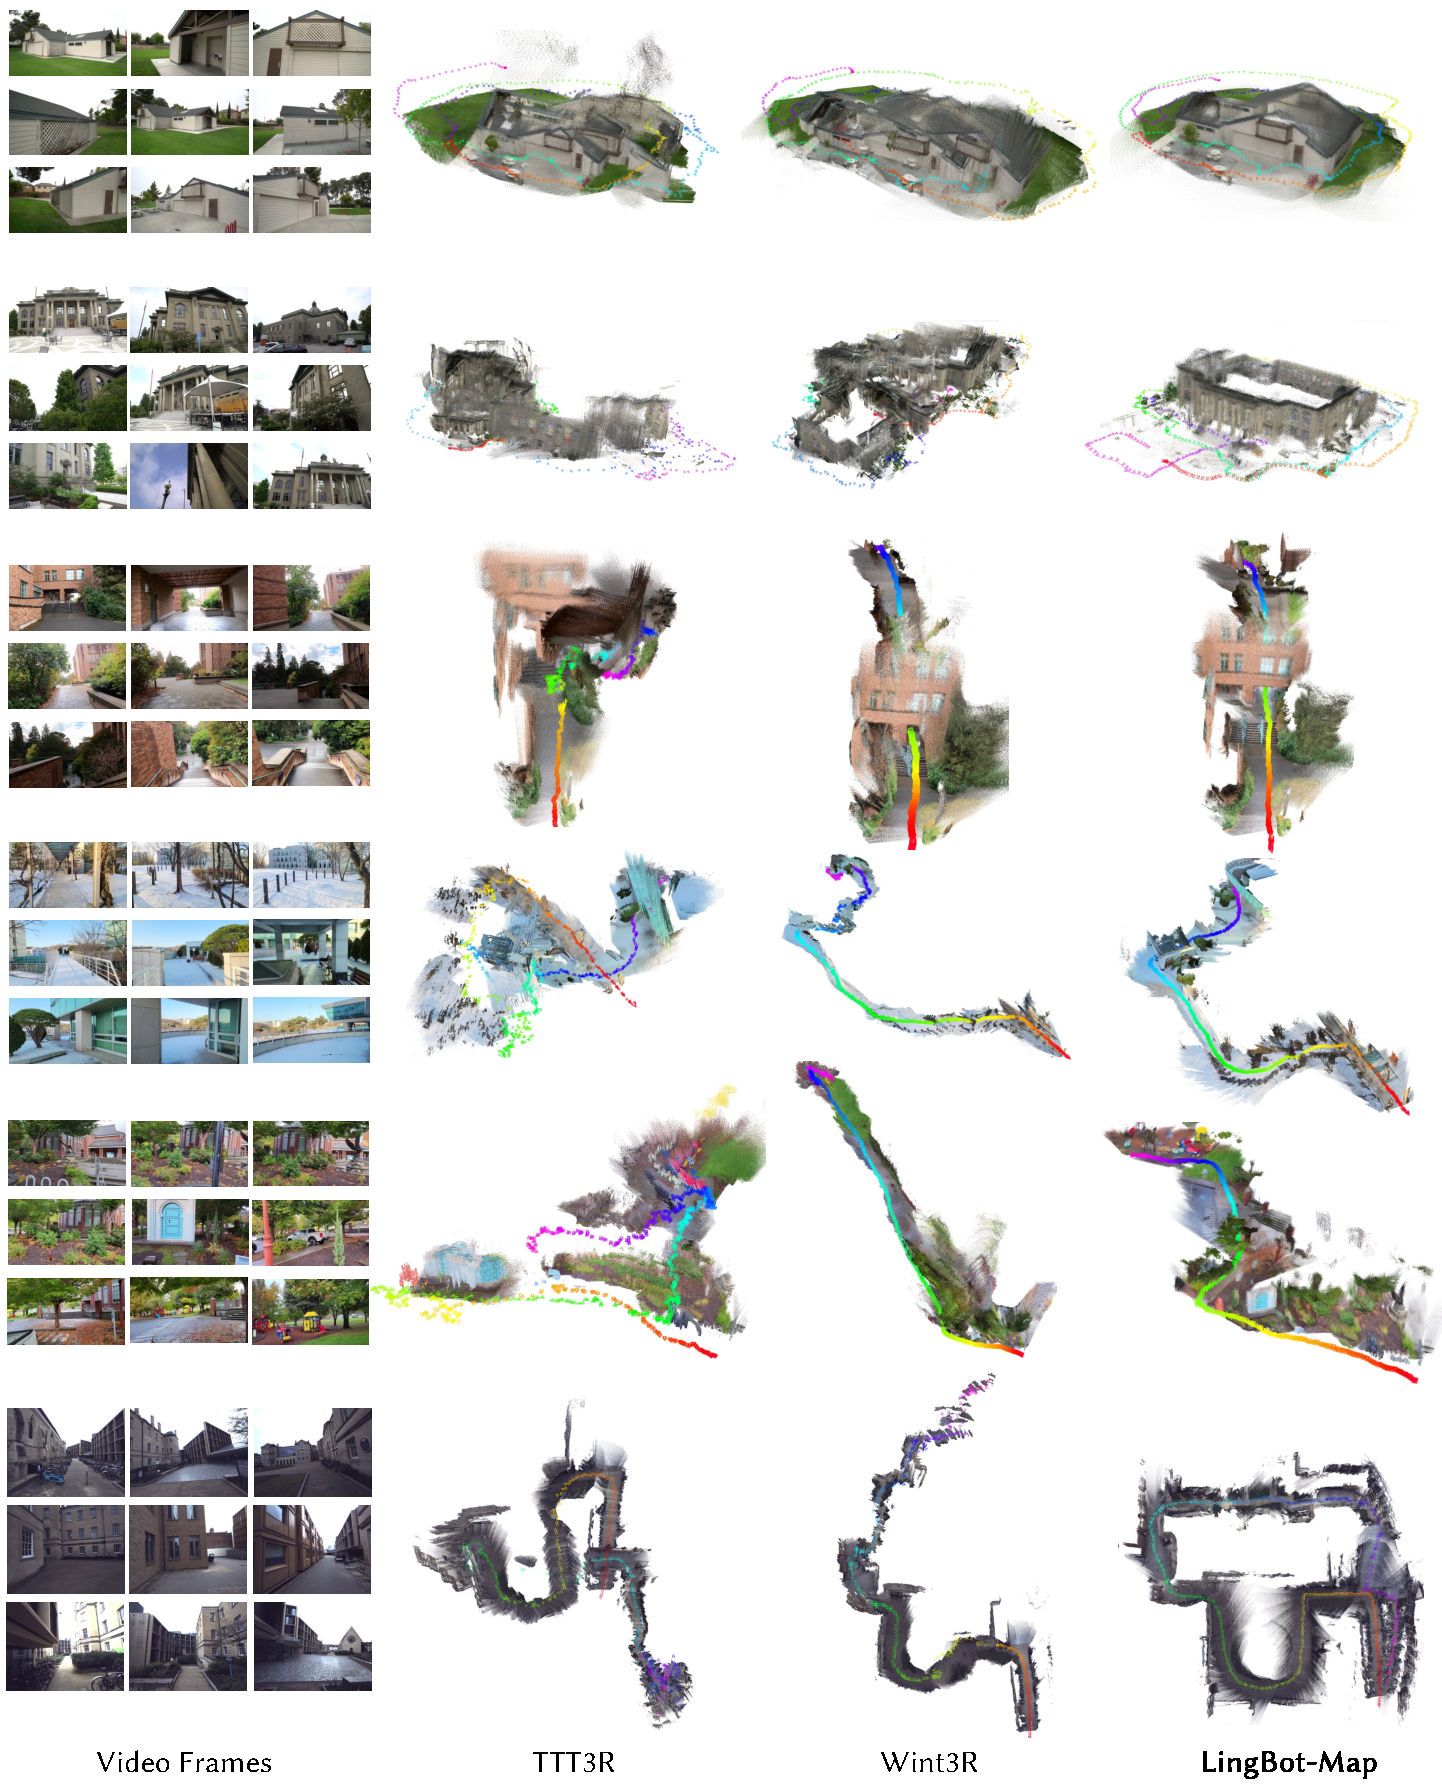
\includegraphics[width=0.98\textwidth]{figures/point_comparison.pdf}

    \caption{\textbf{Qualitative comparison of point cloud reconstruction.}
    LingBot-Map produces geometrically coherent and temporally stable reconstructions, preserving sharp building edges and continuous surfaces even over long sequences with revisits.
    TTT3R and Wint3R suffer from trajectory drift that causes fragmented geometry and duplicated structures, with degradation most severe in complex multi-building scenes (bottom rows).}
    \label{fig:point_comparison}
    \vspace{-1em}
  \end{figure}


\subsection{3D Reconstruction}

We evaluate the 3D reconstruction quality of \method on ETH3D,
7-Scenes, and NRGBD~\cite{azinovic2022neural}.
The evaluation protocol and metrics (Accuracy, Completeness, F1)
are described in~\cref{sec:metrics}.
Quantitative results are summarized in~\cref{tab:pointacc}.

Since reconstruction quality depends directly on pose accuracy
and depth estimation, the improvements reported in the previous
section translate into substantial gains in 3D reconstruction.
\method achieves the best F1 score on all three datasets.
On ETH3D, \method reaches an F1 of 98.98, outperforming the
runner-up Wint3R (77.28) by +21.70 points.
The improvement comes from both better accuracy (0.09 vs.\ 0.28)
and completeness (0.03 vs.\ 0.21), indicating that our
reconstructions are not only more precise but also more complete
in their coverage of the scene.
On 7-Scenes, \method achieves an F1 of 80.39 with the best
accuracy (0.02) and completeness (0.07), matching or exceeding
all baselines.
The gains here are more modest because the room-scale scenes
have limited trajectory length, and most methods already perform
reasonably well; nonetheless, \method still ranks first.
On NRGBD, the advantage is most pronounced: \method achieves an
F1 of 64.26, improving over Wint3R (56.96) by +7.30 points.
NRGBD contains cluttered indoor environments with fine geometric
details, where accumulated pose drift in competing methods leads
to blurred or duplicated surfaces in the reconstruction.
Our drift-resistant trajectory estimation directly benefits
reconstruction fidelity in these scenarios.

A qualitative comparison is shown in~\cref{fig:point_comparison}.
In simpler scenes (top rows), all methods produce reasonable
reconstructions, but TTT3R and Wint3R already show noticeable
misalignment at building edges.
As scene complexity increases (middle rows), competing methods begin
to produce duplicated structures and blurred surfaces, a direct
consequence of accumulated pose drift causing the same geometry to
be projected to different locations.
In the most challenging multi-building outdoor scenes (bottom rows),
the gap becomes striking: TTT3R and Wint3R lose spatial coherence
entirely, producing collapsed and fragmented point clouds where
individual buildings are no longer distinguishable.
In contrast, \method maintains clean geometry with sharp structural
edges and continuous wall surfaces throughout, demonstrating that
the long-range consistency provided by GCA directly translates to
high-fidelity 3D reconstruction.




\begin{table}[t]
\centering
\caption{\textbf{Point cloud reconstruction comparison on ETH3D, 7-Scenes, and NRGBD.} Our method achieves the best results on Accuracy, Completeness, and F1 score. The \textbf{best} and \underline{second best} results are marked.}
\label{tab:pointacc}
\resizebox{\textwidth}{!}{%
\begin{tabular}{l c ccc ccc ccc}
\toprule
\multirow{2}{*}{Methods} & \multirow{2}{*}{Type} &
\multicolumn{3}{c}{ETH3D} &
\multicolumn{3}{c}{7-Scenes} &
\multicolumn{3}{c}{NRGBD} \\
\cmidrule(lr){3-5}\cmidrule(lr){6-8}\cmidrule(lr){9-11}
 &  & Acc $\downarrow$ & Comp $\downarrow$ & F1 $\uparrow$ & Acc $\downarrow$ & Comp $\downarrow$ & F1 $\uparrow$ & Acc $\downarrow$ & Comp $\downarrow$ & F1 $\uparrow$ \\
\midrule
StreamVGGT~\cite{streamVGGT}& online & 0.64 & 0.34 & 58.11 & 0.04 & 0.11 & 69.44 & 0.13 & 0.05 & 45.08 \\
InfiniteVGGT~\cite{yuan2026infinitevggt} & online & 0.65 & 0.35 & 57.69 & 0.04 & 0.11 & 68.53 & 0.13 & 0.05 & 42.27 \\
CUT3R~\cite{cut3r}    & online & 0.57 & 0.50 & 67.63 & 0.07 & 0.10 & 58.98 & 0.25 & 0.15 & 32.22 \\
TTT3R~\cite{chen2025ttt3r} & online & 0.41 & 0.22 & 68.48 & \underline{0.03} & \underline{0.08} & 77.25 & 0.16 & 0.06 & 53.55 \\
Wint3R~\cite{li2025wint3r}      & online & \underline{0.28} & \underline{0.21} & \underline{77.28} & \underline{0.03} & \textbf{0.07} & \underline{78.81} & 0.09 & \underline{0.04} & \underline{56.96} \\
Stream3R~\cite{stream3r2025}      & online & 0.44 & 0.28 & 72.87 & \textbf{0.02} & 0.09 & 78.79 & 0.21 & 0.07 & 54.07 \\
Stream3R-w~\cite{stream3r2025}      & online & 0.58 & 0.37 & 67.09 & 0.04 & 0.15 & 71.94 & 0.20 & 0.06 & 53.74 \\
\method (Ours)      & online & \textbf{0.09} & \textbf{0.03} & \textbf{98.98} & \textbf{0.02} & \textbf{0.07} & \textbf{80.39} & \textbf{0.07} & \textbf{0.03} & \textbf{64.26} \\
\bottomrule
\end{tabular}%
}
\end{table}


\subsection{Ablation Study}
We conduct ablation studies to analyze the contributions of each
component in GCA.
We use TartanAir and TartanGround as the ablation testbed for their
high-quality ground-truth annotations, complex scene geometry, and
long trajectories (up to thousands of frames), which provide a
controlled yet challenging setting that isolates the effect of each
component.
We initialize the model from the first-stage checkpoint and fine-tune
on these datasets, evaluating on the TartanGround validation set
with sequences of 320 frames sampled at a stride of 8 (spanning
${\sim}2{,}400$ frames in temporal extent).
We use a learning rate of $5 \times 10^{-5}$ and follow the same
progressive view curriculum as the main streaming training
(\cref{sec:streaming_training}).
Each ablation experiment requires approximately 3,840 GPU hours.

Results are shown in~\cref{tab:ablation_long_pose}. Starting
from a baseline with only the relative pose loss (row~1), we
progressively add each component and measure its impact.

\paragraph{Anchor Initialization.}
Adding anchor initialization (row~1 $\to$ row~2) boosts AUC@3 from
9.80 to 13.63 (+3.83) and reduces ATE from 8.59 to 7.88.
Monocular streaming reconstruction is inherently scale-ambiguous:
without an explicit geometric reference, the model must implicitly
infer both the coordinate origin and the absolute scale from the
data, which becomes increasingly unreliable as the sequence grows.
The anchor context resolves this by designating the first $n$ frames
as fixed references that establish the scale and coordinate system
before streaming begins.
The improvement in AUC@3 (+3.83) confirms that the anchor mechanism
improves not just global trajectory consistency but also local pose
accuracy, as each new frame can now be registered against a
well-defined geometric reference.

\paragraph{Context Tokens (Trajectory Memory).}
Adding context tokens on top of anchor initialization (row~2 $\to$
row~4) further improves AUC@3 from 13.63 to 15.75 and reduces ATE
from 7.88 to 7.46.
The anchor context and local window together provide a fixed global
reference and dense recent observations, but without any record of
intermediate frames, pose errors accumulate unchecked between the
anchor and the current window.
Context tokens address this by retaining a compact 6-token summary
for each evicted frame, preserving the key geometric cues of the
full observation history at minimal memory cost.
The consistent improvement across all metrics (AUC@3: +2.12,
AUC@30: +1.21, ATE: $-$0.42) validates that even a lightweight
trajectory memory meaningfully reduces long-range drift.

\paragraph{Relative Pose Loss.}
Comparing row~3 (without Rel. Loss) and row~4 (with Rel. Loss)
isolates the effect of relative pose supervision.
Without it, RPE-rot degrades sharply from 2.26 to 5.35
($2.4\times$ worse) and ATE increases from 7.46 to 8.25.
The relative pose loss supervises all frame pairs within the local
pose-reference window, directly constraining the frame-to-frame
relative motion.
This is complementary to the absolute pose loss: while the absolute
loss anchors each frame's pose in the global coordinate system,
the relative loss enforces local geometric consistency within the
sliding window, preventing the small per-frame errors that
compound into trajectory drift over long sequences.
Notably, the rotation degradation ($+$3.09 in RPE-rot) is far more
severe than the translation degradation, suggesting that rotation
estimation is particularly sensitive to the lack of local
pairwise supervision.

\paragraph{Video RoPE.}
The final component, Video RoPE (row~4 $\to$ row~5), yields the
single largest ATE improvement: 7.46 $\to$ 5.98 ($-$1.48), along
with gains across all other metrics (AUC@3: +0.64, AUC@30: +1.95,
RPE-trans: $-$0.15).
Without temporal positional encoding, the trajectory memory tokens
carry geometric information but lack any notion of when each frame
was observed.
Video RoPE injects temporal ordering directly into the attention
computation, enabling the model to reason about the sequential
structure of the trajectory: how far apart two frames are in time,
and in which direction the camera has been moving.
The disproportionately large ATE improvement ($-$1.48 vs.\ the
$-$0.42 from context tokens alone) suggests that temporal ordering
is the missing ingredient that allows the trajectory memory to
realize its full potential for correcting long-range drift.



\begin{table}[t]
\centering
\caption{\textbf{Ablation study on long-sequence pose estimation and trajectory accuracy.}
All components contribute significantly to the final performance. The \textbf{best} results are marked.}
\label{tab:ablation_long_pose}
\begin{tabular}{cccc ccccc}
\toprule
Rel. Loss & A. Init. & Co. Tok. & V. RoPE & AUC@3 $\uparrow$ & AUC@30 $\uparrow$
& ATE $\downarrow$ & RPE-trans $\downarrow$ & RPE-rot $\downarrow$ \\
\midrule
\checkmark &            &            &            & 9.80  & 65.84 & 8.59 & 1.62 & 2.57 \\
\checkmark & \checkmark &            &            & 13.63 & 68.71 & 7.88 & 1.60 & 2.90 \\
           & \checkmark & \checkmark &            & 13.91 & 68.25 & 8.25 & 1.67 & 5.35 \\
\checkmark & \checkmark & \checkmark &            & 15.75 & 69.92 & 7.46 & 1.48 & 2.26 \\
\midrule
\checkmark & \checkmark & \checkmark & \checkmark & \textbf{16.39} & \textbf{71.87}
& \textbf{5.98} & \textbf{1.33} & \textbf{1.93} \\

\bottomrule
\end{tabular}
\end{table}


\paragraph{Pose-Reference Window vs.\ Full Attention.}
Finally, we compare GCA's bounded pose-reference window (size 64)
against full causal attention that retains all historical tokens
(\cref{tab:ablation_sw}).
The pose-reference window yields a $1.7\times$ speedup (11.87 $\to$
20.29 FPS) and a $2.7\times$ memory reduction (36.06 $\to$ 13.28 GB).
More importantly, the bounded window also improves trajectory
accuracy: ATE decreases from 6.60 to 5.98 and RPE-trans from 1.50
to 1.33.
This counterintuitive result can be explained by the fact that
retaining all historical image tokens introduces noise from distant,
less relevant frames that can confuse the attention computation.
GCA's design, which evicts image tokens but preserves compact
context tokens for the full trajectory, retains the essential
geometric cues while filtering out redundant information.
The only metric where full attention leads is RPE-rot (1.71 vs.\
1.93), suggesting that dense historical tokens provide slightly
richer rotational cues at the local level, but this marginal
benefit is far outweighed by the efficiency gains and the improved
global trajectory consistency.
As sequence length grows further, the gap widens: full attention's
memory and compute scale quadratically with the number of frames, while
GCA's cost remains nearly constant (6 tokens per evicted frame),
making it the only viable option for streaming at scale.

\begin{table}[t]
\centering
\caption{\textbf{Pose-reference window (size 64) vs.\ full causal attention.} The bounded window achieves better trajectory accuracy with $1.7\times$ higher speed and $2.7\times$ lower memory. The \textbf{best} and \underline{second best} results are marked.}
\label{tab:ablation_sw}
\begin{tabular}{c|ccc | cc}
\toprule
Window Size  &ATE $\downarrow$ & RPE-trans $\downarrow$ & RPE-rot $\downarrow$ & FPS$\uparrow$ & Mem (GB)$\downarrow$\\
\midrule
64        &\textbf{5.98} & \textbf{1.33}  & \underline{1.93}  &  \textbf{20.29} & \textbf{13.28}\\
Full      & \underline{6.60}  & \underline{1.50} & \textbf{1.71} & \underline{11.87} &  \underline{36.06}\\
\bottomrule
\end{tabular}
\end{table}

